\usetikzlibrary{calc}


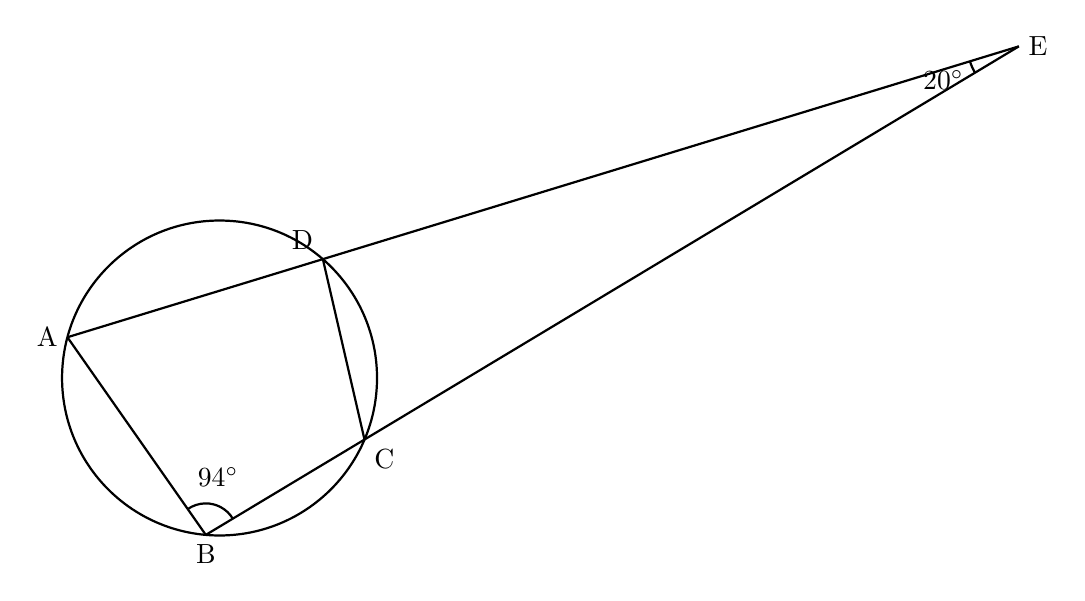
\begin{tikzpicture}[scale=1]

    % Define the radius of the circle to ensure the diagram is well-proportioned
    \def\R{2}
    % Define the center of the circle
    \coordinate (O) at (0,0);

    % Define points A, B, C, D on the circle using polar coordinates.
    % Point B has been shifted left (from 277 to 265).
    \coordinate (A) at (165:\R);
    \coordinate (B) at (265:\R);
    \coordinate (C) at (337:\R);
    \coordinate (D) at (49:\R);

    % Draw the main circle
    \draw[thick] (O) circle (\R);

    % Find point E as the intersection of the extended lines AD and BC
    \coordinate (E) at (intersection of A--{$(A)!5!(D)$} and B--{$(B)!5!(C)$});

    % Draw the lines and segments as shown in the original image
    \draw[thick] (A) -- (B); % Chord AB
    \draw[thick] (C) -- (D); % Chord CD
    \draw[thick] (A) -- (E); % Secant line passing through A, D to E
    \draw[thick] (B) -- (E); % Secant line passing through B, C to E

    % Draw the arc and label for the 94 degree angle at B
    % Recalculated for the new B position: Line BC is at ~31 degrees, line BA is at ~125 degrees
    \draw[thick] (B) ++(31:0.4) arc (31:125:0.4);
    \node at ($(B)+(78:0.75)$) {$94^\circ$};

    % Draw the arc and label for the 20 degree angle at E
    % Recalculated for the new E position: Line ED is at ~197 degrees, line EC is at ~211 degrees
    \draw[thick] (E) ++(197:0.65) arc (197:211:0.65);
    \node at ($(E)+(204:1.05)$) {$20^\circ$};

    % Add text labels for all the geometric points
    \node[left] at (A) {A};
    \node[below] at (B) {B};
    \node[below right] at (C) {C};
    \node[above left] at (D) {D};
    \node[right] at (E) {E};

\end{tikzpicture}